\documentclass[a4paper, 11pt, final, garamond]{book}
\usepackage{cours-preambule}
\usepackage{pdfpages}

\raggedbottom

\makeatletter
\renewcommand{\@chapapp}{Travaux pratiques -- TP}
\makeatother

\let\SavedIndent\indent
\protected\def\indent{%
  \begingroup
    \parindent=\the\parindent
    \SavedIndent
  \endgroup
}
\setlength{\parindent}{0pt}

\begin{document}
\setcounter{chapter}{29}

\chapter{Mesures de champs magnétiques -- Terre et soléno\"ide}
\begin{center}
  \Large
  \textbf{Objectifs}
\end{center}
\begin{itemize}[label=$\diamond$, leftmargin=10pt]
  \item Mesurer différents ordres de grandeurs de champs magnétiques par
    différentes méthodes
\end{itemize}

\section{Mesure du champ magnétique terrestre}
\label{sec:chpT}
\subsection{S'approprier}
\label{ssec:chpTapp}
En première approximation, le champ magnétique terreste équivaut à celui d'un
aimant droit situé au centre de la Terre et dont le pôle Sud pointerait vers le
Nord géographique. L'axe de cet aimant est incliné sur l'axe des pôles
géographiques (correspondant à l'axe de rotation de la Terre sur elle-même) d'un
anglre $\tt_0 \approx \ang{11.5;;}$.
\smallbreak
L'intensité du champ magnétique terrestre est d'environ \SI{5e-5}{T}. Il est
contenu dans un plan vertical passant par les pôles magnétiques terrestres,
appelé \ul{méridien magnétique}. Sa direction fait avec l'horizontal un angle $i$
appelé \ul{inclinaison}, dont la valeur est voisine de \ang{60;;}.

\begin{figure}[h]
  \centering
  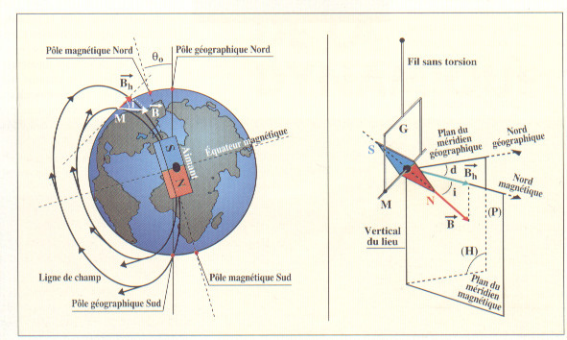
\includegraphics[scale=1]{chpT}
  \label{fig:chpT}
\end{figure}
On possède un dispositif avec une bobine plate et une simple boussole
horizontale posée sur une aiguille~:
\begin{itemize}[label=$\diamond$, leftmargin=10pt]
  \item la boussole n'est sensible qu'à la composante horizontale $\vv{B_h}$ du
    champ magnétique terrestre~;
  \item le champ magnétique $\vv{B}$ créé au centre de la bobine plate
    s'exprime~:
    \[
      \vv{B} = \mu_0 \frac{N}{2R}I \vv{n}
    \]
    avec $N$ le nombre de spires de la bobine, $R$ son rayon, $I$ l'intensité du
    courant qui le traverse, $\vv{n}$ un vecteur normal à la bobine, et $\mu_0 =
    4\pi\times \SI{e-7}{H.m ^{-1}}$ la perméabilité du vide.
\end{itemize}
\noindent
\begin{minipage}[t]{.7\linewidth}
  Le champ magnétique total $\vv{B_{\rm tot}}$ ressenti par la boussole est
  \[
    \vv{B_{\rm tot}} = \vv{B_h} + \vv{B}
  \]
  Lorsque deux champs sont perpendiculaires, on a la relation sur les normes des
  champs~:
  \[
    \tan{\alpha} = \frac{B}{B_h}
  \]
\end{minipage}
\hfill
\begin{minipage}[t]{.25\linewidth}
  ~
  \begin{center}
    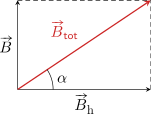
\includegraphics[scale=1]{bh}
    \label{fig:bh}
  \end{center}
\end{minipage}

\subsection{Réaliser et valider}
\label{ssec:chpTreal}

\begin{enumerate}[label=\sqenumi]
  \item Proposer un protocole pour mesurer $B_h$.
  \item Le réaliser et conclure.
\end{enumerate}

\section{Champ magnétique à l'intérieur d'un solénoïde}
\label{sec:sol}
\subsection{S'approprier}
\label{ssec:solapp}
On admet qu'un solénoïde de longueur $L$ et constitué de $N$ spires, parcouru
par un courant d'intensité $I$ génère un champ $\vv{B}$ uniforme en son sein, de
norme $B = \mu_0 \frac{N}{L}I$ avec $\mu_0$ la perméabilité du vide.
\subsection{Réaliser et valider}
\label{ssec:solreal}
\subsubsection{Uniformité du champ magnétique}
\label{sssec:soluni}
On oriente l'axe $\Or x$ du solénoïde positivement de la gauche vers la droite,
l'origine $\Or$ étant placée au centre du solénoïde.
\smallbreak
Un générateur de courant continu réglable est monté en série avec un solénoïde
long et un ampèremètre. Une sonde de \textsc{Hall} coulisse sur son support et
permet de mesurer la valeur du champ magnétique en différents points de l'axe du
solénoïde. On peut sélectionner la composante du champ magnétique à mesurer
($B_x$ ou $B_z$).
\begin{enumerate}
  \item Faire le zéro après avoir placé la sonde au centre la bobine ($x=0$),
    générateur éteint.
  \item Régler le générateur de façon à ce que l'intensité du courant circulant
    dans la bobine soit proche de \SI{2}{A}.
  \item Pour différentes valeurs de $x$, relever la valeur de $B$ indiqué par la
    sonde.
  \sqitem[3] Tracer la courbe de $B$ en fonction de $x$. Dans quel domaine de
  $x$ a-t-on un champ constant à 10\% près~?
\end{enumerate}

\subsubsection{Champ magnétique au centre et nombre de spires}
\label{sssec:solnspires}
On dispose d'un solénoïde dont on peut doubler le nombre de spires $N$, qu'on
branche en série avec un générateur de courant et un ampèremètre.
\begin{enumerate}
  \item Placer la sonde au centre du solénoïde et faire le zéro, générateur
    éteint.
  \item Régler le générateur de façon à ce que l'intensité du courant circulant
    dans la bobine soit proche de \SI{2}{A}. \textbf{Noter sa valeur}, et
    \textbf{vérifier la valeur de l'intensité} avant chaque mesure.
  \sqitem[4] Pour les deux valeurs de $N$ (\num{200} et \num{400}), mesurer la
  valeur de $B$ correspondante. Noter la longueur $L$ du solénoïde. En déduire
  la valeur de $\mu_0$. La comparer à la valeur connue.
\end{enumerate}

\subsubsection{Champ magnétique au centre et intensité du courant}
\label{sssec:solint}
On conserve le nombre de spires maximal (\num{400}) branché en série avec le
générateur de courant continu réglable et l'ampèremètre.
\begin{enumerate}
  \item Mesurer $B$ pour plusieurs valeurs d'intensité.
  \sqitem[5] Tracer la courbe représentant $B$ en fonction de $I$ et l'imprimer.
  \sqitem[6] Effectuer une régression linéaire et en déduire la valeur de
  $\mu_0$. Comparer avec la valeur obtenue précédemment.
\end{enumerate}

\end{document}
